%Chapter
\chapter{Discussion}
\label{chap:chapter1}

%paragraph with reference in bibligraphy.bib
\paragraph{}This paragraph provides a reference to Einstein's paper: \cite{Einstein}. The paragraph also contains an inline equation $a+b=c$.

%Section
\section{Section}
\label{sec:section1}

\paragraph{}This paragraph is located in Chapter~\ref{chap:chapter1} and talks about Figure~\ref{fig:sampleFigureLabel}.

%Figure
\begin{figure}[h]
\centering
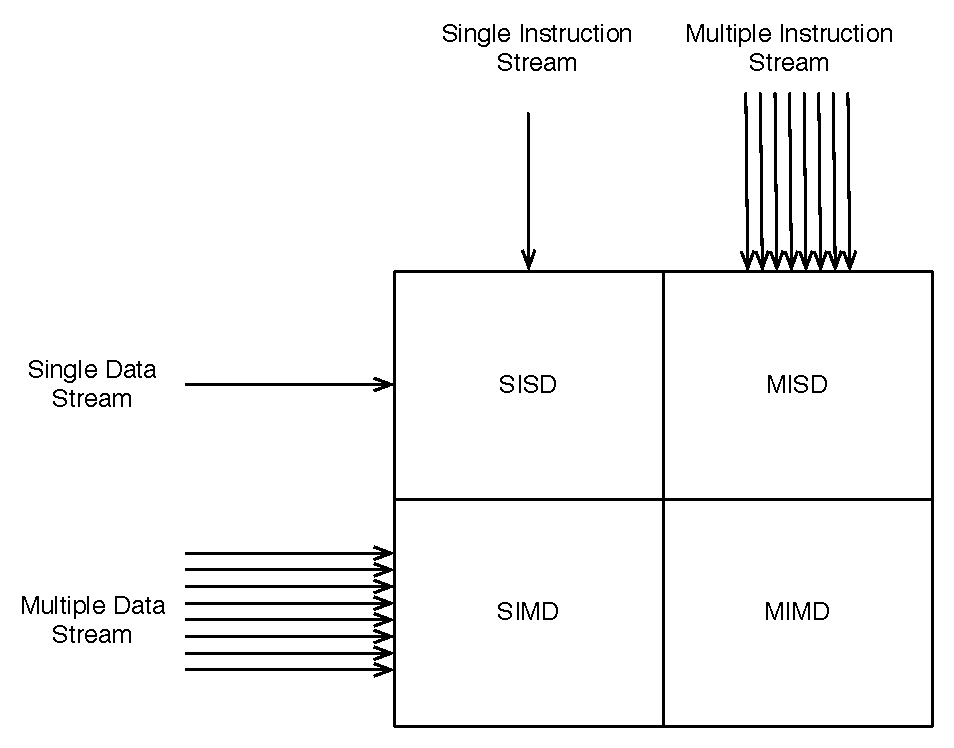
\includegraphics[width=3.5in]{./Figures/sampleFigureFlynn.pdf}
\caption{sample figure caption}
\label{fig:sampleFigureLabel}
\end{figure}

%Subsection
\subsection{Subsection} 
\label{ssec:subsection1}


\paragraph{}This is a paragraph located in a subsection.  This paragraph also reference a  Figure~\ref{fig:sampleFigureLabel}.


%subsection 2
\subsection{Subsection}
\label{ssec:subsection2}

\paragraph{}This paragraph reference another subsection~\ref{sec:section1}.